%%%%%%%%%%%%%%%%%%%%%%%%%%%%%%%%%%%%%%%%%%%%%%%%%%%%%%%%
% Este é um documento que servirá de modelo para
% os relatórios feitos na disciplina Laboratório de Circuitos Lógicos
% 2020-2
%%%%%%%%%%%%%%%%%%%%%%%%%%%%%%%%%%%%%%%%%%%%%%%%%%%%%%%%%

%%%%%%%%%%%%%%%%%%%%%%%%%%%%%%%%%%%%%%%%%%%%%%%%%%%%%%%%%
% Use os diferentes diretórios para colocar os relatórios de cada experimento, deste modo vc consegue manter um histórico e todo material organizado em apenas um local.
% Lembre-se de mudar o Main Document no Menu!!!

\documentclass[12pt]{article}

\usepackage{sbc-template}
\usepackage[brazil]{babel}
\usepackage{graphicx}
\usepackage{url}
\usepackage{float}
\usepackage{listings}
\usepackage{color}
%\usepackage{todonotes}
\usepackage{algorithmic}
\usepackage{algorithm}
\usepackage{hyperref}
\hypersetup{
    colorlinks=true,
    linkcolor=black,
    filecolor=magenta,      
    urlcolor=blue,
    citecolor=black
    }
     
\sloppy

\title{Experimento 3\\ 
Circuitos Combinacionais: Mapa de Karnaugh}

\author{Grupo B2 - Turma 2\\    %%%% LEMBRE-SE DE MUDAR O GRUPO !!!!! %%%%%%
        Allan Victor Almeida Faria, 261010546\\
        Caio César Gonçalves Ribeiro, 211038217\\
        Danilo Alves Ribeiro, 242003754\\
}


\address{Dep. Ciência da Computação -- Universidade de Brasília (UnB)\\
  CIC0231 - Laboratório de Circuitos Lógicos\\
  \today
  \email{allanvictor.almeida@gmail.com, caiocesar20032003@gmail.com,  daniloalvesjob@gmail.com}
}

\begin{document} 
\maketitle

\selectlanguage{american}
 \begin{abstract}
The following work employs mechanisms for simplifying logic functions and circuits, such as 
K-Maps
and modularization and reuse of sub-circuits, to reduce redundancies and
 enable the construction of more compact and efficient combinational electronic circuits.    
\end{abstract}
\selectlanguage{brazil}     
    
 \begin{resumo}
    No seguinte trabalho, utiliza-se mecanismos de simplificação de
    funções e circuitos lógicos, a saber, o Mapa de Karnaugh
    e modularização e reutilização de sub-circuitos, para reduzir
    redundâncias e possibilitar a construção de circuitos eletrônicos
    combinacionais mais compactos e eficientes.
 \end{resumo}


\section{Introdução}
\label{sec:Introducao}

Circuitos reais e efetivos devem dar conta da multiplicidade
e variedade dos fenômenos do mundo, e não só, mais encontrar
relações que possibilitem reduzir redundâncias e fornecer 
soluções mais elegantes para os problemas solucionados
pela eletrônica. Tal necessidade faz com que
os circuitos digitais escalem para muitas variáveis, o que torna
o tratamento de funções por métodos puramente algébricos inescalável. 

\noindent Nesse sentido,
o Mapa de Karnaugh oferece um mecanismo visual (topológico, em uma visão matemática)
para simplificar expressões lógicas, sendo especialmente eficaz no tratamento
de funções de duas a cinco variáveis\cite{wakerly90}. Além dele, a modularização de sub-circuitos
que se comunicam através de uma interface fornece uma maneira de resolver problemas
complexos através de circuitos mais simples. Usaremos os dois mecanismos para
construir circuitos de maioria e minoria, e, ao final, combiná-los.


\subsection{Objetivos}
\label{sec:Objetivos}

\begin{itemize}
    \item Implantar um circuito de maioria usando apenas portas NAND
    \item Projetar e implantar um circuito de minoria utlizando-se de mapas de Karnaugh
    \item Construir um comparador de igualdade vetorial a partir de sub-circuitos modularizados
\end{itemize}

\subsection{Materiais} 
\label{sec:Materiais}
Neste experimento foram utilizados os seguintes materiais e equipamentos:
\begin{itemize}

    \item \textit{Protoboard}
    
    \item Fios

    \item Kit de Eletrônica Digital
    
    \item CIs NAND2, NAND3, NOR2, AND3, NAND4, OR2, NOT
\end{itemize}

\section{Procedimentos e Resultados}
\label{sec:Procedimentos}

Foram montados os três circuitos objetivados no roteiro do experimento.
Nesse sentido, os dois primeiros itens foram combinados para implementação
do terceiro experimento. De modo geral, a alimentação para os circuitos foi
fornecida pelo Kit de Eletrônica, e as saídas foram verificadas com ajuda
visual dos Leds do próprio Kit.

\subsection{Circuito de Maioria}
\label{sec:Mux}

Consiste em um circuito cuja saída
é 1 apenas quando a maior parte das
entradas é 1. Isto é, para um circuito
de quatro entradas, é necessário e suficiente
que três entradas sejam 1:

\begin{equation}
    Y = ABD + ABC + BCD + ACD
\end{equation}

Aplicando o teorema de De Morgan, consegue-se
realizar tal circuito com quatro portas NAND3
e uma NAND4:

\begin{equation}
    Y = \overline{
        \overline{ABD}
        \cdot
        \overline{ABC}
        \cdot
        \overline{BCD}
        \cdot
        \overline{ACD}
    }
\end{equation}


Dessa maneira, o circuito real foi montado assim:

\begin{figure}[H]
    \centering
    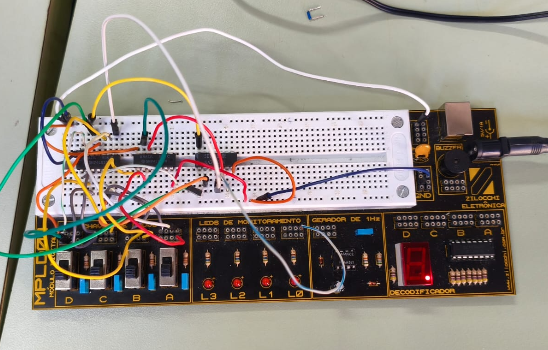
\includegraphics[width=.75\textwidth]{q1real.png}
    \caption{Circuito}
    \label{fig:nand4}
\end{figure}

Feita a simulação, cuja gravação pode ser
vista \href{https://drive.google.com/file/d/10QwYQWrQXRwsCLnVEk2SVldv0WX9bulO/view?usp=drive_link}{aqui}, verificou-se a identidade
entre a tabela teórica e a medida, comprovando 
a corretude do nosso circuito.

\begin{table}[H]
    \centering
    \caption{Tabela Verdade do Circuito de Maioria de 4 Entradas}
    \label{tab:maioria-4-entradas}
    \begin{tabular}{|c|c|c|c|c|}
        \hline
        A & B & C & D & Y \\ \hline
        0 & 0 & 0 & 0 & 0 \\ \hline
        0 & 0 & 0 & 1 & 0 \\ \hline
        0 & 0 & 1 & 0 & 0 \\ \hline
        0 & 0 & 1 & 1 & 0 \\ \hline
        0 & 1 & 0 & 0 & 0 \\ \hline
        0 & 1 & 0 & 1 & 0 \\ \hline
        0 & 1 & 1 & 0 & 0 \\ \hline
        0 & 1 & 1 & 1 & 1 \\ \hline
        1 & 0 & 0 & 0 & 0 \\ \hline
        1 & 0 & 0 & 1 & 0 \\ \hline
        1 & 0 & 1 & 0 & 0 \\ \hline
        1 & 0 & 1 & 1 & 1 \\ \hline
        1 & 1 & 0 & 0 & 0 \\ \hline
        1 & 1 & 0 & 1 & 1 \\ \hline
        1 & 1 & 1 & 0 & 1 \\ \hline
        1 & 1 & 1 & 1 & 1 \\ \hline
    \end{tabular}
\end{table}

\subsection{Circuito de Minoria}

Consiste em um circuito cuja saída é 1
apenas quando a maior parte das entradas é
0. Pode-se deduzir a expressão mínima a partir
da tabela verdade:

\begin{table}[H]
    \centering
    \caption{Tabela Verdade do Circuito de Decisão de Minoria}
    \label{tab:minoria}
    \begin{tabular}{|c|c|c|c|c|}
        \hline
        D & C & B & A & Y \\ \hline
        0 & 0 & 0 & 0 & 1 \\ \hline
        0 & 0 & 0 & 1 & 1 \\ \hline
        0 & 0 & 1 & 0 & 1 \\ \hline
        0 & 0 & 1 & 1 & 0 \\ \hline
        0 & 1 & 0 & 0 & 1 \\ \hline
        0 & 1 & 0 & 1 & 0 \\ \hline
        0 & 1 & 1 & 0 & 0 \\ \hline
        0 & 1 & 1 & 1 & 0 \\ \hline
        1 & 0 & 0 & 0 & 1 \\ \hline
        1 & 0 & 0 & 1 & 0 \\ \hline
        1 & 0 & 1 & 0 & 0 \\ \hline
        1 & 0 & 1 & 1 & 0 \\ \hline
        1 & 1 & 0 & 0 & 0 \\ \hline
        1 & 1 & 0 & 1 & 0 \\ \hline
        1 & 1 & 1 & 0 & 0 \\ \hline
        1 & 1 & 1 & 1 & 0 \\ \hline
    \end{tabular}
\end{table}

Da tabela, podemos preencher o mapa de Karnaugh
para chegar na expressão mínima:


\begin{figure}[H]
    \centering
    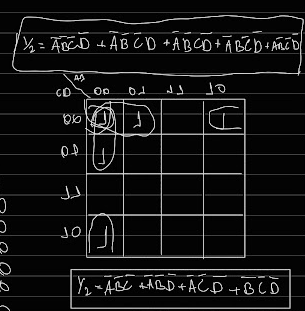
\includegraphics[width=.5\textwidth]{karnaugh.png}
    \caption{Expressão minimizada}
    \label{fig:karnaugh}
\end{figure}

\begin{equation}
    Y_2 =
    \overline{D}\,\overline{C}\,\overline{B}
    + \overline{D}\,\overline{C}\,\overline{A}
    + \overline{D}\,\overline{B}\,\overline{A}
    + \overline{C}\,\overline{B}\,\overline{A}
\end{equation}


A partir disso, foi montado o circuito físico e também
gravado o preenchimento da tabela verdade \href{https://drive.google.com/file/d/1kZFUdpag3f2Ry3ZOJtsxl__zzS4Iap4R/view?usp=drive_link}{aqui},
o qual revelou a identidade entre a tabela verdade teórica e mensurada, determinando que nosso circuito
satisfaz as condições para ser um circuito de decisão de minoria.

\begin{figure}[H]
    \centering
    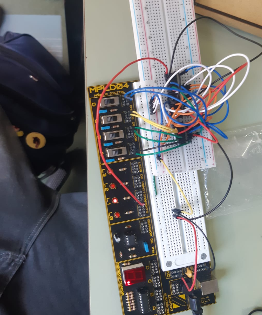
\includegraphics[width=.5\textwidth]{q2real.png}
    \caption{Circuito montado}
    \label{fig:q2}
\end{figure}

\subsection{Circuito de Igualdade}

Consiste em circuito cuja saída é 1 apenas
quando o número de 0's e 1's nas entradas
é igual. Tal condição equivale, nesse contexto,
a situação em que ambas as saídas dos circuitos de maioria
e minoria são 0. Basta processarmos as saídas por uma porta NOR
para obtermos o resultado.

\begin{equation}
    Y = \overline{Y_1 + Y_2}
\end{equation} 

O circuito foi montado, como dito anteriormente, combinando os circuitos anteriores,
contudo, não foi possível gravar a medição devido à falta de tempo, embora - dada a 
simplicidade da solução - estejamos seguros da corretude do experimento.

\begin{figure}[H]
    \centering
    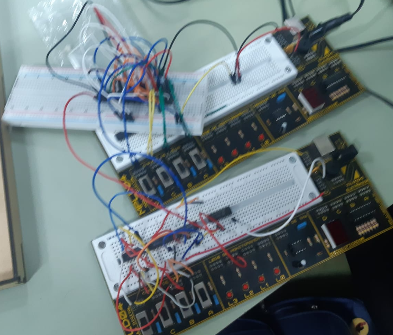
\includegraphics[width=.5\textwidth]{q3real.png}
    \caption{Circuito montado}
    \label{fig:q3}
\end{figure}

\section{Conclusões}
\label{sec:Conclusao}

Os experimentos realizados corresponderam à teoria. A utilização de mapas de Karnaugh
provou-se aliada na simplificação do segundo circuito, comprovando assim sua aplicação
na realidade. Devido a falta de tempo, o grupo não conseguiu gravar os resultados
do terceiro experimento, embora a corretude dos experimentos antecessores dê uma boa
garantia da validade deste.

\bibliographystyle{plain}
\bibliography{relatorio}  %Aqui é a definição do arquivo .bib a ser usado pelas referências


\newpage 
% Colocar aqui apenas as respostas dos itens da Auto-Avaliação
\section*{Auto-Avaliação}

\begin{enumerate}
    \item b
    \item d
    \item c
    \item a
    \item d
\end{enumerate}


\end{document}
